\documentclass{article}
\usepackage[english]{babel}
\usepackage[utf8]{inputenc}
\usepackage[T1]{fontenc}
\usepackage{hyperref}
\usepackage[margin=0.5in]{geometry}
\usepackage{xspace}
\usepackage{xcolor}
\usepackage{amsmath}
\usepackage{graphicx}
\usepackage{palatino}
\usepackage{microtype}

\title{What Is Hop-Skip-Jump?}
\author{Drew Dolgert}
\date{\today}


\begin{document}
\maketitle

\section{Introduction}
The hop-skip-jump model was introduced in X as a simplest model
of dynamic invasion to include multiscale movement behavior.
The model is a heuristic version of, ``all I can say is that the
vector moves more quickly in this range than outside this range.''
Statistically speaking, this kind of heuristic becomes a
maximum entropy distribution.

We are interested in dynamical spread of insects in complex
urban environments. There can be subtly-different versions of
even so simple a model, so we ask here which versions are
most appropriate to use for our main tasks, estimation and
inference.

What are the mechanisms for spread, ignoring observation
or removal from a house?
\begin{enumerate}
  \item A within-house insect population model leads to a rate of
insects leaving either with people or by themselves.
  \begin{enumerate}
    \item Growth Model
    \begin{enumerate}
      \item Logistic growth, which is called Beverton-Holt in discrete time
      \item Ricker, chaotic
      \item Representation of logistic or chaotic with MaxEnt distributions for transfer among discrete levels
    \end{enumerate}
    \item State representation for the house population
    \begin{enumerate}
      \item Binary---Infected or not infected.
      \item Multiple discrete levels---Low, medium, high
      \item Continuous
    \end{enumerate}
  \end{enumerate}
  \item Three kinds of dispersal mechanisms from the house.
    \begin{enumerate}
    \item A dispersal model for insects determines a transmission rate
to neighboring houses.
    \begin{enumerate}
      \item Walk/flight models for Triatoma.
      \item Uniform within a cutoff distance (for a given metric)
      \item Kernel-based
    \end{enumerate}
    \item A movement model for people
determines spread over short and long distances.
    \begin{enumerate}
      \item Within-cutoff distance versus outside of it.
      \item Kernel-based
    \end{enumerate}
    \item There
is also the possibility of importation from outside the domain.
This is often included in order to exclude zero-likelihood
events in an inference.
    \begin{enumerate}
      \item Usually a constant value.
      \item Could be seasonal.
    \end{enumerate}
    \end{enumerate}
  \item Once an insect arrives at a house, there is, from the
within-house model, a possibility for survival of the population
past the initial hazard of failure to infest.
\end{enumerate}


\section{Continuous-time Discrete Space Models}
A model which explicitly includes insects has a slightly
different meaning from one which represents house-to-house
transmission.

Define a bug model, where the state of a house is defined
by how many bug tokens are at the house. Zero bugs is uninfected.
Movement from one house to another moves a bug. Bugs multiply
at a house and may die off stochastically.

How does a house-to-house infection model compare with a bug
model? A house can be in a susceptible state or an infected
state. For this model, infection represents the ability to
infect another house. Is a house infected when the first bug
arrives? It seems more reasonable to assign a house an
infected state when it has passed the likelihood of stochastic
die-off.

In this second model, the infection transition, where one
house infects another, represents not only movement
of the bug but the likelihood that the bug establishes itself.
The $I$ state is not an infected state but an infectious state.
The hazard rate, over time, for an infected house to change
the status of its neighbor includes not only the time
for travel of the bug but also time for establishment of the
new population in the next house.

For a bug model, a bug can move from an infected house to
another infected house. It just changes the count of bugs.
For a house-to-house model, the transition of the neighboring
house to being infectious has already happened.
Disabling the possibility of infecting a neighboring house
in a simple SIR model doesn't equate to stopping the bugs
from moving. It just means the house can't become more infectious
when it is already infectious.


\section{Movement Model}
There are a few choices to make about a movement model, mostly
concerning normalization.

One basic question is what the two rates of movement represent.
Is there a farther movement that is mostly human-mediated 
and a local movement that is mostly insect-mediated?
Or is a significant portion of local movement human-mediated,
so that the hop represents a sum of skipping plus a raw hop rate?


\subsection{Conservation in English}
The state of both models is houses on a landscape, where
each is either infested or not infested. Ignoring
observation and recovery, let's focus on a susceptible-infected
kind of process. At each time step, $T_n$, each infected house
has a hazard rate for infecting any other house, which we label
by infecting house, $i$, target susceptible, $j$, and time step
$n$, as $\beta_{ij}(T_n)$. This hazard rate can be normalized per
infectious house. It can be normalized over the number of neighbors,
or it can be unnormalized, as explained below.

Which makes physical sense, normalization or not?
The hazard rate for infection, $\beta$, represents not just whether
a vector leaves but whether it both leaves and successfully infests
the destination house. When we picture steps of the vector leaving,
wandering, arriving, setting up shop in the new place, they
all factor into a single $\beta$, which is a hazard rate for
a state change in the neighboring house, given an infected
state in the source house. The binary state of a house being
infected or not infected probably isn't decided strictly according
to whether a single individual vector arrived but whether
the initial importation can survive past the early time stochastic
die-off.

Let's walk through what we might believe.
\begin{enumerate}
  \item The rate of vectors leaving a house should be determined
        by the carrying capacity, which we might set at a uniform
        value to start. For wandering insects, this makes sense.
        For insects hitching a ride on people, is this still true,
        or do people leave more often when there are more neighbors?
  \item Wandering insects are more likely to find a good home if there
        are more houses as neighbors. A single neighbor or an infested
        house is more likely to receive an importation than a house
        among many neighbors of an infested house.
  \item Closer neighbors, because they receive more importations,
        are more likely to survive early time stochastic die-off.
\end{enumerate}
For jumps, it seems conservation of hazard represents the notion
that people in a house travel only so often. For hops, conservation
represents the idea that bugs are good at walking or flying towards
light.

The multiscale model is about two processes, spread by people and
spread by vector locomotion. Within hop distance, locomotion
dominates. The synthetic likelihood paper uses separate conservation
for the two length scales, which says that the two processes
happen with separate likelihoods.

\subsection{Conservation in Math}
The simplest form of hop-skip-jump states that the hazard rate
for infecting a house depends only on the distance to that
house, so
\begin{equation}
  \beta_{ij}(T_n)=\beta_h\quad\mbox{or}\quad \beta_j,
\end{equation}
where $\beta_h$ is for hops and $\beta_j$ is for jumps. This is a
limited form of a distance kernel. Given a distance $r_{ij}$
between houses, a pure distance kernel would be
\begin{equation}
  \beta_{ij}(T_n)=\beta(r_{ij}).
\end{equation}
A consequence of the bare hazard rates is that the total hazard
rate for vectors leaving a host depends on the number of
neighbors,
\begin{equation}
  \sum_j \beta_{ij}(T_n)=\sum_j\beta(r_{ij}).
\end{equation}
More insects leave houses with more neighbors. This is the model
used currently for the Jewell-type inference on invasions.

We could, instead, normalize the number of insects to leave,
retaining an \emph{orientation preference\/} for where they go.
The normalization, $\gamma$ would come from the total hazard rate for leaving
a house,
\begin{equation}
  \sum_j \gamma\beta_{ij}(T_n)=\gamma\sum_j\beta(r_{ij})\equiv \beta_i(T_n).
\end{equation}
This leads to a normalization
\begin{equation}
  \gamma_i(T_n)=\beta_i(T_n)/\sum_j\beta(r_{ij})
\end{equation}
on the hazard rates. Note that the total hazard for leaving a house
can depend on the house and the time step.
This first form of conservation of vectors is not what we use.

Instead, the work with synthetic likelihood conserves vector dispersal
for each of the two main types, vectors leaving the house themselves versus
vectors carried by people. Using $n_h$ as the number of neighbors in hopping
distance and $n_{ij}$ as the number of neighbors in jumping distance of $i$,
\begin{eqnarray}
  n_{ih} \gamma_{ih}\beta_h& =&\beta_i\phi \\
  n_{ij} \gamma_{ij}\beta_j&= &\beta_i(1-\phi)
\end{eqnarray}
Solving for the hazard rate for transmission to any one neighbor gives
\begin{eqnarray}
  \gamma_{ih}\beta_h& =&\beta_i\phi/n_{ih} \\
  \gamma_{ij}\beta_j&= &\beta_i(1-\phi)/n_{ij}
\end{eqnarray}
For uniform grids, the counts of neighbors won't change, but they
could be interesting on city landscapes. Note that the hazards listed
here are not exactly those used in the synthetic likelihoods paper
because of complications about random importation and a probability
for failure of an importation to surivive stochastic die-off in
the infested house.

There could be a third way to normalize. Use one normalization for
spread by travel of people and a separate normalization for locomotion.
Instead of having a hop hazard and jump hazard, have a uniform
travel-any-distance by people hazard and a hop-by-vector hazard
which has a cutoff distance. It's the sum of two normalized, kernel-based
models.

\subsection{Note on Maximum Entropy}
The classic maximum entropy distribution to express ``it happened between
this time and this time'' is a uniform distribution. For continuous-time
stochastic simulation, the equivalent maximum entropy isn't a uniform
distribution but an exponential distribution, with uniform hazard rate.
I have a citation which explains this, but it stems from simulation
as being about the probability of something happening given that it has
not yet happened.


\section{Bug Counts}
Is there some way to increase the amount of knowledge we have about
the system by incorporating bug counts? The state of the house wouldn't
be infested or not infested but would include some estimate of the level
of infestation. Counts are an observation process on top of the model
for how the bugs increase over time.

\subsection{Models for Bug Growth}
The two models under consideration are a Ricker model and some form
of logistic growth.

The Ricker model is a discrete time model for the density of individuals,
of the form
\begin{equation}
  N_{n+1}=N_n\exp\left[r(1-N_n/K\right]
\end{equation}
where $r$ is growth rate and $K$ carrying capacity.

Logistic growth is pretty standard. The deterministic form is
\begin{equation}
N(t)=\frac{N_0Ke^{rt}}{K+N_0(e^{rt}-1)}.
\end{equation}
It's the solution to the differential equation
\begin{equation}
  \frac{dN}{dt}=r\left(1-N/K\right)N
\end{equation}
The discrete form of this is called Beverton-Holt.

Rewriting this to conform to a logistic equation shows
its shape,
\begin{equation}
N(t)=\frac{K}{1+\exp\left(-rt+\ln(K/N_0-1)\right)}
\end{equation}
\begin{equation}
N(t)=\frac{K}{1+\exp\left(-r(t-\ln(K/N_0-1)/r)\right)}
\end{equation}
Carrying capacity is $K$.
The steepness of the curve is $r$, and its midpoint
is $\ln(K/N_0-1)/r$. Having an estimate $t_0$ for
the time when the bugs are halfway to carrying capacity
sets a relation $K/N_0=1+e^{rt_0}$. This is important because
we have a better sense for half-carrying capacity than other parameters.

This is equivalent to a birth rate $\beta(1-N/K)$ and death rate $\delta$
in a well-mixed population for a stochastic, continuous-time model.
Another kind of solution makes the differential equation stochastic
as an Ito process. Another odd way to treat bug levels as stochastic
is to model the growth rate, $r$, as a random variable and 
use random variable transformation (RVT) to obtain a resulting
stochastic value for $N(t)$.

\subsection{Inclusion of Bug Counts in the Model}
The data is the number of bugs observed in each house, a number
usually below ten but rarely near two hundred. We would like to include
this information in an inference of the sort Jewell described, so
it's part of a continuous-time likelihood.

Any variation in a continuous-time stochastic model happens in
one of three places.
\begin{enumerate}
  \item Change the state of the system by changing the discrete
        places.
  \item Change the state of the system by changing representation
        of the tokens. These can be discrete or continuous.
  \item Change the distribution associated with a transition.
\end{enumerate}

An obvious atomistic-style model includes a token for each bug.
This simplifies construction of a simulation, but it greatly
increases the state space, which might make inference harder
rather than easier. Imagine an MCMC where the number of bugs
per house is a parameter.

If we think of logistic growth as deterministic, then the number
of bugs since infection is known, and it just scales the total
hazard rate, $\beta_i$ for bugs leaving the house. In the MCMC inference,
there would still be only one parameter per house, the time
of infection. The hazard for infecting neighbors, however,
would follow a logistic growth, so it requires numerical integration.
Having a time-dependent hazard rate would also require root-finding
in a non-exponential continous-time solver. This is doable, just
more complicated. The total hazard for bugs to leave is $\beta_i$
and the parameter for bug hazard is $\beta_0$. $T_i$ is time of
infection for the house.
\begin{equation}
  \beta_i(T)=\beta_0N(T-T_i)
\end{equation}

Another option is to discretize the infection level of a house in 
some way that is informative about how long ago the house
was infested. If we give a house three levels, then we could 
identify a hazard rate for movement from one level to the next
by performing stochastic simulations of bug growth and then using
survival analysis to determine rates for house movement to the
next state. This makes the infection process for neighboring
houses look simpler, but the rate for movement among infection
stages could be non-exponential unless we approximate with an exponential.

Let's work through the math of a particular case. We imagine that
there are an infinite number of recovered states, one for each bug count.
This is OK in Gillespie if handled as a separate draw within a
hierarchical direct method. The point is that we observe the count of bugs
at the moment we see the house is recovered. From this count we want
to estimate when the house was infected. We don't use the bug count
in any other place during simulation. It's just there for inference.
Mathematically, that's $P(n_o | T_r-T_i)$. This comes in two pieces,
the probability of a number of bugs and the probability of the observing
a certain number. By the law of total probability, that's
\begin{equation}
  P(n_o|T_r-T_i)=\sum_{n_b}P(n_o|n_b)P(n_b|T_r-T_i)
\end{equation}
For the observation process, we can use a Poisson process.
For the number of bugs, given the time, we have a bunch of
options, as above. In a situation like this, ensuring 
sufficient expression of our lack of surety seems a good call.
We could simulate it stochastically (throwing away those trajectories
which collapse early), or find a closed form solution, which I cannot
guess.

Once we decide on $P(n_o|T_r-T_i)$, then we can simulate the
infestation process with our typical continuous-time SIR
and annotate it after the fact with a number of bugs at each place,
given the period of infection for an individual house.
This happens, in this case, not to violate Gillespie because there
can be no conflicts about this transition with enabling other
transitions.

Once we have a $P(n_o|T_r-T_i)$ that we like, what we need for
inference is $P(T_r-T_i|n_o)$.
\begin{equation}
  P(T_r-T_i|n_o)P(n_o)=P(n_o|T_r-T_i)P(T_r-T_i)
\end{equation}
Oh, look, it's Bayes' rule. This will give us the pdf to use
in a likelihood for MCMC.


\section{Excess Growth}
If we assume logistic growth for the count of bugs in a house
and make that a deterministic number, then a theoretically
simple hazard rate for bugs leaving a house is excess growth,
which is the difference between exponential growth and logistic growth.

\begin{figure}
\centerline{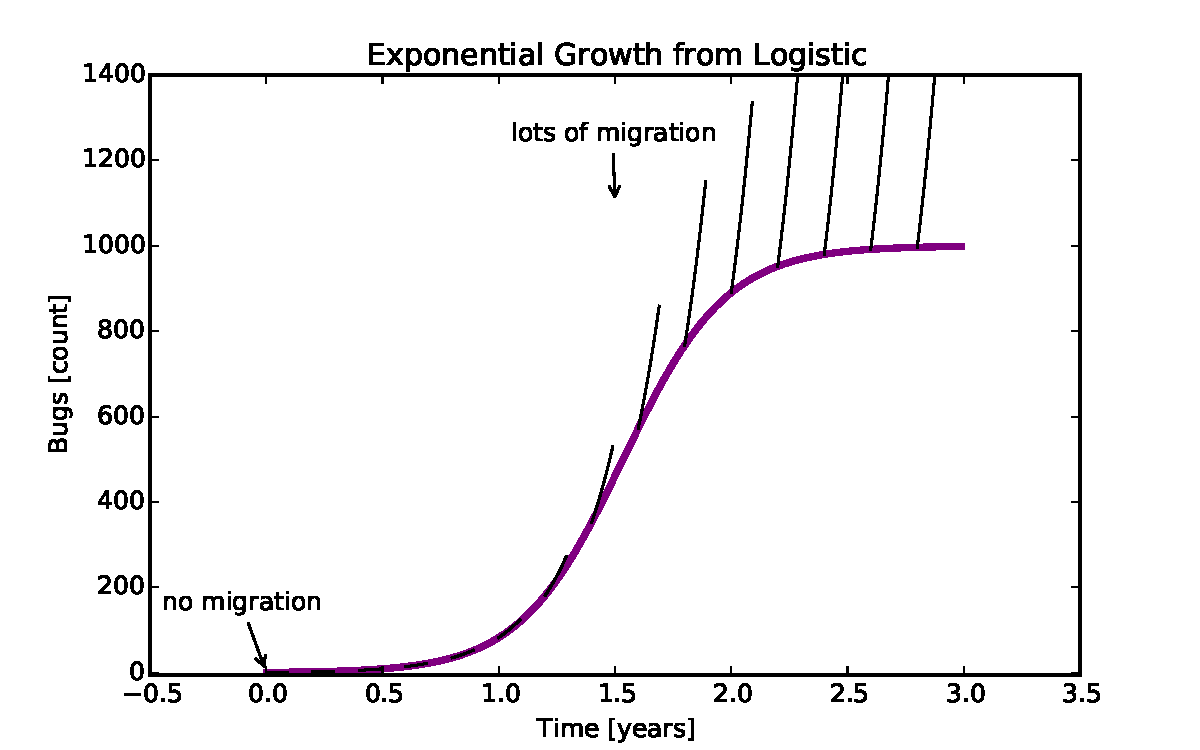
\includegraphics[width=10cm]{excess}}
\caption{The total number of bugs in a house follows
a logistic model. The growth rate per bug is constant.
Excess growth is assumed to contribute to migration.
Parameters are $N_0=1\:\mbox{bugs}$, $r=4.5\:\mbox{bugs/bug--yr}$, $K=1000\:\mbox{bugs}.$\label{fig:excessslopes}}
\end{figure}

Exponential growth is
\begin{equation}
  \frac{dN'}{dt}=rN,
\end{equation}
where $r$ is the growth rate and $N$ is the bug count.
The $N$ on the right is not $N'$. It comes instead from logistic
growth. The hazard for bugs leaving is the difference in the
rate of growth for each, or
\begin{equation}
  \frac{d(N'-N)}{dt}=rN-r\left(1-\frac{N}{K}\right)N=rN^2/K
\end{equation}
Writing out $N$ for logistic growth, this hazard is
\begin{eqnarray}
  \lambda(t)dt&\equiv & \frac{d(N'-N)}{dt} \\
  & = & \frac{r}{K}\left[
  \frac{N_0Ke^{rt}}{K+N_0(e^{rt}-1)}\right]^2dt \\
  &=&rN_0^2K\left[
    \frac{e^{rt}}{K+N_0(e^{rt}-1)}\right]^2dt
\end{eqnarray}
The time $t=T-T_e$ is a time since enabling.

Stochastic sampling requires an integral of the hazard
and the inverse of the integral of the hazard. Are these possible
in closed form?

We want to integrate this hazard. Let's make a couple of things simpler
with $rt\equiv t'$ and $K=N_0K'$.
\begin{eqnarray}
  \lambda(t)dt & = & \lambda(t'/r)dt'/r \\
  &=&rN_0^2K\left[
    \frac{e^{t'}}{K+N_0(e^{t'}-1)}\right]^2dt'/r \\
  &=&N_0^2K\left[
    \frac{e^{t'}}{K+N_0(e^{t'}-1)}\right]^2dt' \\
  &=&N_0^2(N_0K')\left[
    \frac{e^{t'}}{N_0K'+N_0(e^{t'}-1)}\right]^2dt' \\
  &=&N_0^2(N_0K')\frac{1}{N_0^2}\left[
    \frac{e^{t'}}{K'+(e^{t'}-1)}\right]^2dt' \\
  & = & N_0K'\left[\frac{e^{t'}}{K'+e^{t'}-1}\right]^2dt'.\label{eqn:hazardrescale} \\
  & = & N_0K'\left[\frac{1}{1+e^{-t'}(K'-1)}\right]^2dt'
\end{eqnarray}
Because time is always greater than or equal to zero, and carrying
capacity is positive, the denumerator is greater than zero.
The factor $K'$ is greater than one, so we might write the denumerator
to show that.
\begin{equation}
  \lambda(t)dt =N_0K'\left[\frac{e^{t'}}{e^{t'}+(K'-1)}\right]^2dt'
\end{equation}

Let's make a substitution such that
\begin{eqnarray}
  e^{t'}+(K'-1)& = & (u + 1)(K'-1) \\
  e^{t'} & = & u(K'-1) \\
  e^{t'}dt' & = & du(K'-1) \\
  u(K'-1)dt' & = & du(K'-1) \\
  dt' & = & (1/u)du
\end{eqnarray}
Returning to the main equation,
\begin{eqnarray}
  \lambda(t)dt & = & K\left[\frac{u(K'-1)}{(u+1)(K'-1)}\right]^2
      \frac{du}{u} \\
  & = & K\frac{u}{(u+1)^2}du \\
\end{eqnarray}

Sometimes these are easier when split, so
this gets integrated by parts, using two fractions
\begin{equation}
 \frac{u}{(u+1)^2}=\frac{A}{(u+1)^2} + \frac{B}{u+1}
\end{equation}
Puttering says the answer is
\begin{equation}
 \frac{u}{(u+1)^2}=\frac{-1}{(u+1)^2} + \frac{1}{u+1}.
\end{equation}
This integrates to
\begin{equation}
  \int_{u_0}^{u_1}\frac{u}{(u+1)^2}du=\left.-\frac{u}{u+1} + \ln(u+1)\right|_{u_0}^{u_1}.
\end{equation}
The integral of the hazard, in terms of $u(t)$ and replacing $N_0K'=K$, is then
\begin{equation}
  \int_{u_0(t)}^{u_1(t)}\lambda(t)dt=K\left[
    \ln\left(\frac{u_1+1}{u_0+1}\right)-\frac{u_1-u_0}{(u_0+1)(u_1+1)}
    \right].
\end{equation}
Now reverse substitutions. Derive here some handy quantities.
\begin{eqnarray}
  u & = & \frac{e^{t'}}{K'-1} \\
    & = & \frac{e^{rt}}{K/N_0 - 1} \\
    & = & \frac{N_0e^{rt}}{K-N_0} \\
  u\frac{K-N_0}{N_0} & = & e^{rt} \\
  t & = & \frac{1}{r}\ln\left[\frac{u(K-N_0)}{N_0}\right] \\
    & = & \frac{1}{r}\ln\left[u((K/N_0)-1)\right] \\
  u + 1 & = & \frac{N_0e^{rt}+K-N_0}{K-N_0} \\
        & = & \frac{K + N_0(e^{rt}-1)}{K-N_0} \\
  \frac{u}{u+1} & = & \frac{N_0e^{rt}}{K + N_0(e^{rt}-1)}
\end{eqnarray}
In code, the transformation between $u$ and $t$
looks like \href{https://github.com/adolgert/hop-skip-bite/blob/0ea11efae867e209c90aeab8c087c749ec52a2f7/hopskip/src/excess_growth.hpp#L141-L142}{this}.



In code, the two calculations are integrated hazard and
its inverse.
The implicit integral is
\begin{equation}
  x_a=\int_{T_0}^{T_1}\lambda(s)ds.
\end{equation}
Again, convert from $T$ to $u$, and solve, this time numerically,
\begin{equation}
  \frac{x_a}{K}+\ln(u_0+1)-\frac{u_0}{u_0+1}=\ln(u_1+1)-\frac{u_1}{u_1+1}.
\end{equation}
The left-hand side will be known, and the right-hand side is the unknown.
Once $u_1$ is found, convert to a time using $t=(1/r)\ln(u(K/N_0-1))$.
The Brent solver needs lower and upper bounds for its solution. The lower
bound would be $u_0$. The upper bound we might take from
labeling the left-hand side $x_a'$ and raising both sides
by $e$ to get
\begin{equation}
 e^{x_a'}=(u_1+1)e^{-u_1/(u_1+1)}.
\end{equation}
The right-hand side's exponential is between 1 and $1/e$, so the maximum
value of $u_1$ is $u_1=\exp(x_a' + 1)-1$.

What happens for solving the inverse integral when the time difference
is small? This matters because roundoff error for small differences
can cause roots to be on the same side of zero, so Brent's method fails.
\begin{eqnarray}
  \int_{u_0(t)}^{u_1(t)}\lambda(t)dt& =& K\left[
    \ln\left(\frac{x+u_0+1}{u_0+1}\right)-\frac{x}{(u_0+1)(x+u_0+1)}
    \right] \\
  x_a/K & = & \ln\left(1+\frac{x}{u_0+1}\right)-\frac{x}{(u_0+1)(x+u_0+1)} \\
  & = & \frac{x}{u_0+1}-\frac{x^2}{2(u_0+1)^2}-\frac{x}{(u_0+1)(x+u_0+1)} \\
  & = & \frac{x(x+p)}{p(x+p)}-\frac{x}{p(x+p)} \\
  & = & \frac{x^2 +(p-1)x}{p(x+p)} \\
  (x_a/K)p(x+p) & =&  x^2 +(p-1)x \\
  0 & = & x^2 + (p-1-px_a/K)x - p^2x_a/K \\
  x & = & \frac{-(p-1-px_a/K)\pm\sqrt{(p-1-px_a/K)^2+4p^2x_a/K}}{2} \\
  x & = & \frac{-(u_0-(1+u_0)x_a/K)\pm\sqrt{(u_0-px_a/K)^2+4(1+u_0)^2x_a/K}}{2} \\
\end{eqnarray}
This doesn't work. Mistake somewhere.


Maybe a simple way to approximate the integral is
to use a Riemann sum. Take
\begin{eqnarray}
  \int_{u_0(t)}^{u_0(t)+\Delta u}\lambda(t)dt& \approx& K\frac{u_0}{(u_0+1)^2}
      \Delta u \\
  \Delta u&=& \frac{x_a(u_0+1)^2}{Ku_0} \\
\end{eqnarray}
This one works.


Is this a good time to remind ourselves that we don't want the
excess growth rate but a scaled excess growth rate? It corresponds
to death of bugs on their way to the next house. It's just a factor
on the integral and on $x_a$ for the inverse integral.
What does it mean to add a scale to the hazard rate?

The free parameters of the system, $N_0$, $K$, and $r$
can be seen in Eq.~\ref{eqn:hazardrescale}. The
$r$ parameter is a scaling on the time. $K/N_0$
appears in transformations from $u$ to $t$ and back.
$K$, not $K'$, then appears in front of the equation as an overall
scaling on the hazard rate. This means that changing scaling
to reflect the death of bugs is equivalent to changing
$K$ while keeping $K/N_0$ fixed.

The maximum hazard rate, for large times, is
\begin{equation}
  \lambda_{\mbox{\tiny max}}=rK.
\end{equation}
For the parameters in Fig.~\ref{fig:excessslopes}, this value is
4,500/year. That means infecting the neighbor a dozen times a day.
We want to dial that down.
Here's how we set parameters.
\begin{enumerate}
  \item Estimate $t_0$, the time to half capacity, from field
        observation, expert opinion.
  \item Set $r$ from studies on individuals.
  \item Use the constitutive equation $K'=1+e^{rt_0}$ to
        determine $K'$.
  \item Don't worry about $N_0$ because we then decide
        how long we think it would take a house at carrying
        capacity to infect a neighbor. Call this hazard
        $\beta$. Work backwards $p$ in
        to get $prK=\beta$, so $p=\beta/(rK)$.
\end{enumerate}
I expect sensitivity to $r$ and $K'$ to be lower. They
just set the shape of the curve.



%%%%%%%%%%%%%%%%%%%%%%%%%%%%%%%%%%%%%%%%%%%%%%%%
\section{Discrete Bug Counts}
The main reference for stochastic models at the bug level
is N{\aa}sell\cite{Nasell2001}. Let's first discuss a single household.
The state of the house is $n$, the current number of bugs.
Given $n$, the birth rate and death rate are
\begin{eqnarray}
  \lambda_n & = & \lambda\left(1-\alpha_1\frac{n}{N}\right)n \\
  \mu_n & = & \mu\left(1+\alpha_2\frac{n}{N}\right)n
\end{eqnarray}
with the caveat that, at $n=N$, the birth rate is defined at zero.
This makes the system bounded. $N$ is not the carrying capacity.
The parameters are then $N$, $\lambda$, $\mu$, $\alpha_1$, and $\alpha_2$.

The assumption earlier was that the rate of infestation of
neighbors is proportional to the excess growth rate, which is
$\lambda\alpha_1n^2/N$. Two different ways to understand this
are as a heuristic or as a microscopic model. The heuristic assumes
that excess growth rate results in a higher hazard rate for infestation
of neighbors, meaning the probability of infestation given that the
neighbors aren't yet infested. This excludes re-infestation, or adding
bugs to a house that already has bugs. The microscopic model
sees bugs as leaving one house, dying at a rate, and arriving at neighbors.
In this case, having multiple infested neighbors increases the chance
that early infestation survives stochastic die-off.

The basic beginning question is what values of parameters for
a single house with bugs correspond to a logistic model with the given
parameters. This system will have $R_0=\lambda/\mu>1$. In this
case, the carrying capacity is
\begin{equation}
  K_1=\frac{R_0-1}{\alpha_1 R_0+\alpha_2}N.
\end{equation}
The variance on carrying capacity is related to the $\alpha$s,
\begin{equation}
  \sigma_1=\frac{\sqrt{(\alpha_1+\alpha_2)R_0}}{\alpha_1R_0+\alpha_2}\sqrt{N}.
\end{equation}
N{\aa}sell's examples use $\alpha_1=1$ and $\alpha_2=0$. 
Fixing this choice would fix variance in the distribution, given birth
and death rates to determine $R_0$. If there were data on stochastic die-off,
it would inform the choice of these parameters.

Do we know the growth rate, $r$? Compared to the microscopic model,
$r=\mu(R_0-1)=\lambda-\mu$. What is measured in the lab is closer to $\lambda$.
Try fixing $\alpha_1=1$ and $\alpha_2=0$. Then
\begin{equation}
  K_1=\frac{R_0-1}{R_0}N=\frac{\lambda-\mu}{\lambda}N.
\end{equation}

You tell me $K_1=1000$ and $r=4.5$. I'll make a rule
of thumb that $R_0=\lambda/\mu=1.5$. Then $r=\mu(1.5-1)=\mu/2$,
so $\mu=2r$ That means $\lambda=3r$. As well,
$N=K_1 R_0/(R_0-1)=K_1 (3/2)/(1/2)=3K_1$.


\begin{figure}
\centerline{\includegraphics[width=10cm]{bug_trajectory.pdf}}
\caption{Trajectories from a Verhulst simulation of one
house. Parameters are equivalent to
$N_0=20\:\mbox{bugs}$, $r=4.5\:\mbox{bugs/bug--yr}$, $K=1000\:\mbox{bugs}.$\label{fig:bug_trajectory}}
\end{figure}

\bibliographystyle{plain}
\bibliography{hopskip}
\end{document}
